\subsection{二叉树的简单应用:Huffman编码}

\begin{frame}
    \frametitle{\insertsubsectionhead}
    \begin{exampleblock}{哈夫曼(Huffman)编码}
        \begin{itemize}
            \item 需求:信息传输中的压缩编码
                \begin{itemize}
                    \item 频率\alert{高}的信息采用\alert{短}编码
                    \item 频率\alert{低}的信息采用\alert{长}编码
                \end{itemize}
            \item 目标:用尽可能少的数据表示尽可能多的信息
            \item 应用:语音、图像、视频等流媒体数据的压缩
        \end{itemize}
    \end{exampleblock}
\end{frame}

\begin{fragile}
    \frametitle{\insertsubsectionhead}
    \bicolumns[0.5]{
        \begin{table}
            \small
            \centering
            \caption{例:两种颜色二进制编码的总数据量比较}
            \label{tab:demo_huffman_lena}
            \begin{tabular}{c|rr|r}
                \toprule
                \textbf{颜色} & \textbf{定长} & \textbf{Huffman} & \textbf{出现概率} \\
                \midrule
                $A$ & \texttt{000} & \texttt{00} & $18\%$ \\
                $B$ & \texttt{001} & \texttt{11} & $32\%$ \\
                $C$ & \texttt{010} & \texttt{010} & $10\%$ \\
                $D$ & \texttt{011} & \texttt{100} & $14\%$ \\
                $E$ & \texttt{100} & \texttt{101} & $16\%$ \\
                $F$ & \texttt{101} & \texttt{0110} & $4\%$ \\
                $G$ & \texttt{110} & \texttt{0111} & $6\%$ \\
                \midrule
                \textbf{总数据量}\footnotemark & \alert{$3n$} & \alert{$2.6n$} & \\
                \bottomrule
            \end{tabular}
        \end{table}
    }{
        \begin{figure}
            \centering
            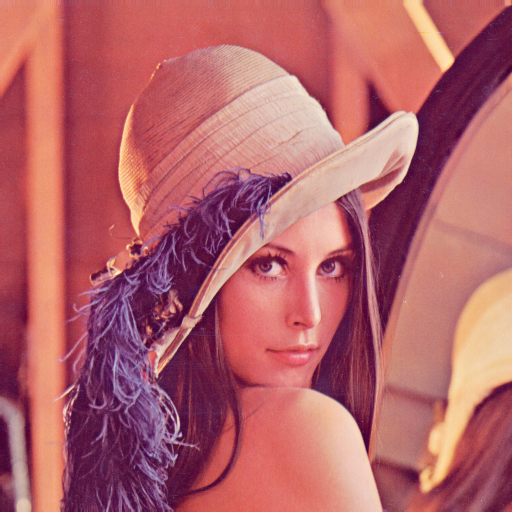
\includegraphics[width=0.8\textwidth]{images/lena.png}
            \caption{实例图片}
            \label{fig:lena}
        \end{figure}   
    }

    \footnotetext{$n$为像素点个数}
\end{fragile}

\begin{fragile}
    \frametitle{\insertsubsectionhead}
    \bicolumns[0.4]{
        \begin{block}{问题转化与建模}
            \begin{itemize}
                \item 因二进制编码,故二叉树表示
                \item 左、右子树路径分别表示0与1
                \item 编码值与叶结点一一对应
                \item 叶结点记录编码值对应权重
                \item 其他结点表示其子结点权重和
                \item 根至叶路径表示该叶对应编码
            \end{itemize}
        \end{block}
    }{
        \begin{figure}
            \centering
            \begin{tikzpicture}[ >=stealth, thick, black!50, %
                    list item/.style={draw=gray, circle, thick}, %
                    level distance=4ex, %
                    level/.style={sibling distance=28ex/#1}
                ]
                \node [nonterminal] {$100$}
                    child [dotted] {node [nonterminal,solid] {$38$}
                        child [dotted] {node [terminal,solid] {$A|18$}}
                        child [solid] {node [nonterminal] {$20$}
                            child [dotted] {node [terminal,solid] {$C|10$}}
                            child [solid] {node [nonterminal] {$10$}
                                child [dotted] {node [terminal,solid] {$F|4$}}
                                child [solid] {node [terminal] {$G|6$}}
                            }
                        }
                    }
                    child [solid] {node [nonterminal] {$62$}
                        child [dotted] {node [nonterminal,solid] {$30$}
                            child [dotted] {node [terminal,solid] {$D|14$}}
                            child [solid] {node [terminal] {$E|16$}}
                        }
                        child [solid] {node [terminal] {$B|32$}}
                    };
            \end{tikzpicture}
            \caption{Huffman编码树示例\footnotemark}
            \label{fig:demo_huffman_tree}
        \end{figure}
    }

    \footnotetext{路径中虚线表示0,实线表示1}
\end{fragile}

\begin{frame}
    \frametitle{\insertsubsectionhead}
    \begin{block}{Huffman编码的目标}
        \begin{itemize}
            \item 最小化所有叶结点深度的加权线性组合,即
                \[
                    \min_{}{\sum_{k=0}^{n-1}{\omega_{k}d_{k}}}
                \]
                其中$\omega_{k}$与$d_{k}$分别为第$k$个叶结点的\alert{权重}与
                \alert{深度}
            \item 满足上述要求的最优二叉树被称为相应信息的Huffman编码树
        \end{itemize}
    \end{block}
\end{frame}

\begin{frame}
    \frametitle{\insertsubsectionhead}
    \begin{block}{Huffman编码树的构建过程}
        \begin{enumerate}
            \item \textbf{初始化}:由给定的权重集合$\{\omega_{k}\}_{k=0}^{n-1}$
                  构建由$n$棵根树组成的\alert{森林}$\mathcal{F}$
            \item \textbf{合并}:在$\mathcal{F}$中选取根权重\alert{最小}的两棵二
                  叉树分别作为左右子树构建新二叉树
            \item \textbf{替换}:以新二叉树替换两棵旧二叉树
            \item \textbf{重复}:重复步骤2、3直至$\mathcal{F}$中只有一棵二叉树即
                  为Huffman编码树
        \end{enumerate}
    \end{block}
\end{frame}

\begin{fragile}
    \frametitle{\insertsubsectionhead}
    \begin{figure}
        \centering
        \begin{subfigure}[T][0.45\textheight][b]{0.1\textwidth}
            \centering
            \begin{tikzpicture}[ >=stealth, thick, black!50, %
                    list item/.style={draw=gray, circle, thick}, %
                    level distance=4ex, %
                    level/.style={sibling distance=28ex/#1}
                ]
                \node [terminal] {$A|18$};
            \end{tikzpicture}
            \caption{$A$}
            \label{subfig:demo_huffman_1a}
        \end{subfigure}
        ~
        \begin{subfigure}[T][0.45\textheight][b]{0.1\textwidth}
            \centering
            \begin{tikzpicture}[ >=stealth, thick, black!50, %
                    list item/.style={draw=gray, circle, thick}, %
                    level distance=4ex, %
                    level/.style={sibling distance=28ex/#1}
                ]
                \node [terminal] {$B|32$};
            \end{tikzpicture}
            \caption{$B$}
            \label{subfig:demo_huffman_1b}
        \end{subfigure}
        ~
        \begin{subfigure}[T][0.45\textheight][b]{0.1\textwidth}
            \centering
            \begin{tikzpicture}[ >=stealth, thick, black!50, %
                    list item/.style={draw=gray, circle, thick}, %
                    level distance=4ex, %
                    level/.style={sibling distance=28ex/#1}
                ]
                \node [terminal] {$C|10$};
            \end{tikzpicture}
            \caption{$C$}
            \label{subfig:demo_huffman_1c}
        \end{subfigure}
        ~
        \begin{subfigure}[T][0.45\textheight][b]{0.1\textwidth}
            \centering
            \begin{tikzpicture}[ >=stealth, thick, black!50, %
                    list item/.style={draw=gray, circle, thick}, %
                    level distance=4ex, %
                    level/.style={sibling distance=28ex/#1}
                ]
                \node [terminal] {$D|14$};
            \end{tikzpicture}
            \caption{$D$}
            \label{subfig:demo_huffman_1d}
        \end{subfigure}
        ~
        \begin{subfigure}[T][0.45\textheight][b]{0.1\textwidth}
            \centering
            \begin{tikzpicture}[ >=stealth, thick, black!50, %
                    list item/.style={draw=gray, circle, thick}, %
                    level distance=4ex, %
                    level/.style={sibling distance=28ex/#1}
                ]
                \node [terminal] {$E|16$};
            \end{tikzpicture}
            \caption{$E$}
            \label{subfig:demo_huffman_1e}
        \end{subfigure}
        ~
        \begin{subfigure}[T][0.45\textheight][b]{0.1\textwidth}
            \centering
            \begin{tikzpicture}[ >=stealth, thick, black!50, %
                    list item/.style={draw=gray, circle, thick}, %
                    level distance=4ex, %
                    level/.style={sibling distance=28ex/#1}
                ]
                \node [terminal] {\alert{$F|4$}};
            \end{tikzpicture}
            \caption{$F$}
            \label{subfig:demo_huffman_1f}
        \end{subfigure}
        ~
        \begin{subfigure}[T][0.45\textheight][b]{0.1\textwidth}
            \centering
            \begin{tikzpicture}[ >=stealth, thick, black!50, %
                    list item/.style={draw=gray, circle, thick}, %
                    level distance=4ex, %
                    level/.style={sibling distance=28ex/#1}
                ]
                \node [terminal] {\alert{$G|6$}};
            \end{tikzpicture}
            \caption{$G$}
            \label{subfig:demo_huffman_1g}
        \end{subfigure}
        \caption{Huffman编码树构建过程:初始化}
        \label{fig:demo_huffman_construction_1}
    \end{figure}
\end{fragile}

\begin{fragile}
    \frametitle{\insertsubsectionhead}
    \begin{figure}
        \centering
        \begin{subfigure}[T][0.45\textheight][b]{0.1\textwidth}
            \centering
            \begin{tikzpicture}[ >=stealth, thick, black!50, %
                    list item/.style={draw=gray, circle, thick}, %
                    level distance=4ex, %
                    level/.style={sibling distance=28ex/#1}
                ]
                \node [terminal] {$A|18$};
            \end{tikzpicture}
            \caption{$A$}
            \label{subfig:demo_huffman_2a}
        \end{subfigure}
        ~
        \begin{subfigure}[T][0.45\textheight][b]{0.1\textwidth}
            \centering
            \begin{tikzpicture}[ >=stealth, thick, black!50, %
                    list item/.style={draw=gray, circle, thick}, %
                    level distance=4ex, %
                    level/.style={sibling distance=28ex/#1}
                ]
                \node [terminal] {$B|32$};
            \end{tikzpicture}
            \caption{$B$}
            \label{subfig:demo_huffman_2b}
        \end{subfigure}
        ~
        \begin{subfigure}[T][0.45\textheight][b]{0.1\textwidth}
            \centering
            \begin{tikzpicture}[ >=stealth, thick, black!50, %
                    list item/.style={draw=gray, circle, thick}, %
                    level distance=4ex, %
                    level/.style={sibling distance=28ex/#1}
                ]
                \node [terminal] {\alert{$C|10$}};
            \end{tikzpicture}
            \caption{$C$}
            \label{subfig:demo_huffman_2c}
        \end{subfigure}
        ~
        \begin{subfigure}[T][0.45\textheight][b]{0.1\textwidth}
            \centering
            \begin{tikzpicture}[ >=stealth, thick, black!50, %
                    list item/.style={draw=gray, circle, thick}, %
                    level distance=4ex, %
                    level/.style={sibling distance=28ex/#1}
                ]
                \node [terminal] {$D|14$};
            \end{tikzpicture}
            \caption{$D$}
            \label{subfig:demo_huffman_2d}
        \end{subfigure}
        ~
        \begin{subfigure}[T][0.45\textheight][b]{0.1\textwidth}
            \centering
            \begin{tikzpicture}[ >=stealth, thick, black!50, %
                    list item/.style={draw=gray, circle, thick}, %
                    level distance=4ex, %
                    level/.style={sibling distance=28ex/#1}
                ]
                \node [terminal] {$E|16$};
            \end{tikzpicture}
            \caption{$E$}
            \label{subfig:demo_huffman_2e}
        \end{subfigure}
        \begin{subfigure}[T][0.45\textheight][b]{0.2\textwidth}
            \centering
            \begin{tikzpicture}[ >=stealth, thick, black!50, %
                    list item/.style={draw=gray, circle, thick}, %
                    level distance=4ex, %
                    level/.style={sibling distance=6ex/#1}
                ]
                \node [nonterminal] {\alert{$10$}}
                    child [dotted] {node [terminal,solid] {$F|4$}}
                    child [solid] {node [terminal] {$G|6$}};
            \end{tikzpicture}
            \caption{$F+G$}
            \label{subfig:demo_huffman_2fg}
        \end{subfigure}
        \caption{Huffman编码树构建过程:合并与替换}
        \label{fig:demo_huffman_construction_2}
    \end{figure}
\end{fragile}

\begin{fragile}
    \frametitle{\insertsubsectionhead}
    \begin{figure}
        \centering
        \begin{subfigure}[T][0.45\textheight][b]{0.1\textwidth}
            \centering
            \begin{tikzpicture}[ >=stealth, thick, black!50, %
                    list item/.style={draw=gray, circle, thick}, %
                    level distance=4ex, %
                    level/.style={sibling distance=28ex/#1}
                ]
                \node [terminal] {$A|18$};
            \end{tikzpicture}
            \caption{$A$}
            \label{subfig:demo_huffman_3a}
        \end{subfigure}
        ~
        \begin{subfigure}[T][0.45\textheight][b]{0.1\textwidth}
            \centering
            \begin{tikzpicture}[ >=stealth, thick, black!50, %
                    list item/.style={draw=gray, circle, thick}, %
                    level distance=4ex, %
                    level/.style={sibling distance=28ex/#1}
                ]
                \node [terminal] {$B|32$};
            \end{tikzpicture}
            \caption{$B$}
            \label{subfig:demo_huffman_3b}
        \end{subfigure}
        ~
        \begin{subfigure}[T][0.45\textheight][b]{0.3\textwidth}
            \centering
            \begin{tikzpicture}[ >=stealth, thick, black!50, %
                    list item/.style={draw=gray, circle, thick}, %
                    level distance=4ex, %
                    level/.style={sibling distance=12ex/#1}
                ]
                \node [nonterminal] {$20$}
                    child [dotted] {node [terminal,solid] {$C|10$}}
                    child [solid] {node [nonterminal] {$10$}
                        child [dotted] {node [terminal,solid] {$F|4$}}
                        child [solid] {node [terminal] {$G|6$}}
                        };
            \end{tikzpicture}
            \caption{$C+F+G$}
            \label{subfig:demo_huffman_3cfg}
        \end{subfigure}
        ~
        \begin{subfigure}[T][0.45\textheight][b]{0.1\textwidth}
            \centering
            \begin{tikzpicture}[ >=stealth, thick, black!50, %
                    list item/.style={draw=gray, circle, thick}, %
                    level distance=4ex, %
                    level/.style={sibling distance=28ex/#1}
                ]
                \node [terminal] {\alert{$D|14$}};
            \end{tikzpicture}
            \caption{$D$}
            \label{subfig:demo_huffman_3d}
        \end{subfigure}
        ~
        \begin{subfigure}[T][0.45\textheight][b]{0.1\textwidth}
            \centering
            \begin{tikzpicture}[ >=stealth, thick, black!50, %
                    list item/.style={draw=gray, circle, thick}, %
                    level distance=4ex, %
                    level/.style={sibling distance=28ex/#1}
                ]
                \node [terminal] {\alert{$E|16$}};
            \end{tikzpicture}
            \caption{$E$}
            \label{subfig:demo_huffman_3e}
        \end{subfigure}
        \caption{Huffman编码树构建过程:合并与替换}
        \label{fig:demo_huffman_construction_3}
    \end{figure}
\end{fragile}

\begin{fragile}
    \frametitle{\insertsubsectionhead}
    \begin{figure}
        \centering
        \begin{subfigure}[T][0.45\textheight][b]{0.1\textwidth}
            \centering
            \begin{tikzpicture}[ >=stealth, thick, black!50, %
                    list item/.style={draw=gray, circle, thick}, %
                    level distance=4ex, %
                    level/.style={sibling distance=28ex/#1}
                ]
                \node [terminal] {\alert{$A|18$}};
            \end{tikzpicture}
            \caption{$A$}
            \label{subfig:demo_huffman_4a}
        \end{subfigure}
        ~
        \begin{subfigure}[T][0.45\textheight][b]{0.1\textwidth}
            \centering
            \begin{tikzpicture}[ >=stealth, thick, black!50, %
                    list item/.style={draw=gray, circle, thick}, %
                    level distance=4ex, %
                    level/.style={sibling distance=28ex/#1}
                ]
                \node [terminal] {$B|32$};
            \end{tikzpicture}
            \caption{$B$}
            \label{subfig:demo_huffman_4b}
        \end{subfigure}
        ~
        \begin{subfigure}[T][0.45\textheight][b]{0.3\textwidth}
            \centering
            \begin{tikzpicture}[ >=stealth, thick, black!50, %
                    list item/.style={draw=gray, circle, thick}, %
                    level distance=4ex, %
                    level/.style={sibling distance=12ex/#1}
                ]
                \node [nonterminal] {\alert{$20$}}
                    child [dotted] {node [terminal,solid] {$C|10$}}
                    child [solid] {node [nonterminal] {$10$}
                        child [dotted] {node [terminal,solid] {$F|4$}}
                        child [solid] {node [terminal] {$G|6$}}
                        };
            \end{tikzpicture}
            \caption{$C+F+G$}
            \label{subfig:demo_huffman_4cfg}
        \end{subfigure}
        ~
        \begin{subfigure}[T][0.45\textheight][b]{0.24\textwidth}
            \centering
            \begin{tikzpicture}[ >=stealth, thick, black!50, %
                    list item/.style={draw=gray, circle, thick}, %
                    level distance=4ex, %
                    level/.style={sibling distance=6ex/#1}
                ]
                \node [nonterminal] {$30$}
                    child [dotted] {node [terminal,solid] {$D|14$}}
                    child [solid] {node [terminal] {$E|16$}};
            \end{tikzpicture}
            \caption{$D+E$}
            \label{subfig:demo_huffman_4de}
        \end{subfigure}
        \caption{Huffman编码树构建过程:合并与替换}
        \label{fig:demo_huffman_construction_4}
    \end{figure}
\end{fragile}

\begin{fragile}
    \frametitle{\insertsubsectionhead}
    \begin{figure}
        \centering
        \begin{subfigure}[T][0.45\textheight][b]{0.5\textwidth}
            \centering
            \begin{tikzpicture}[ >=stealth, thick, black!50, %
                    list item/.style={draw=gray, circle, thick}, %
                    level distance=4ex, %
                    level/.style={sibling distance=18ex/#1}
                ]
                \node [nonterminal] {$38$}
                    child [dotted] {node [terminal,solid] {$A|18$}}
                    child [solid] {node [nonterminal] {$20$}
                        child [dotted] {node [terminal,solid] {$C|10$}}
                        child [solid] {node [nonterminal] {$10$}
                            child [dotted] {node [terminal,solid] {$F|4$}}
                            child [solid] {node [terminal] {$G|6$}}
                        }
                    };
            \end{tikzpicture}
            \caption{$A+C+F+G$}
            \label{subfig:demo_huffman_5acfg}
        \end{subfigure}
        ~
        \begin{subfigure}[T][0.45\textheight][b]{0.1\textwidth}
            \centering
            \begin{tikzpicture}[ >=stealth, thick, black!50, %
                    list item/.style={draw=gray, circle, thick}, %
                    level distance=4ex, %
                    level/.style={sibling distance=28ex/#1}
                ]
                \node [terminal] {\alert{$B|32$}};
            \end{tikzpicture}
            \caption{$B$}
            \label{subfig:demo_huffman_5b}
        \end{subfigure}
        ~
        \begin{subfigure}[T][0.45\textheight][b]{0.24\textwidth}
            \centering
            \begin{tikzpicture}[ >=stealth, thick, black!50, %
                    list item/.style={draw=gray, circle, thick}, %
                    level distance=4ex, %
                    level/.style={sibling distance=6ex/#1}
                ]
                \node [nonterminal] {\alert{$30$}}
                    child [dotted] {node [terminal,solid] {$D|14$}}
                    child [solid] {node [terminal] {$E|16$}};
            \end{tikzpicture}
            \caption{$D+E$}
            \label{subfig:demo_huffman_5de}
        \end{subfigure}
        \caption{Huffman编码树构建过程:合并与替换}
        \label{fig:demo_huffman_construction_5}
    \end{figure}
\end{fragile}

\begin{fragile}
    \frametitle{\insertsubsectionhead}
    \begin{figure}
        \centering
        \begin{subfigure}[T][0.45\textheight][b]{0.5\textwidth}
            \centering
            \begin{tikzpicture}[ >=stealth, thick, black!50, %
                    list item/.style={draw=gray, circle, thick}, %
                    level distance=4ex, %
                    level/.style={sibling distance=18ex/#1}
                ]
                \node [nonterminal] {\alert{$38$}}
                    child [dotted] {node [terminal,solid] {$A|18$}}
                    child [solid] {node [nonterminal] {$20$}
                        child [dotted] {node [terminal,solid] {$C|10$}}
                        child [solid] {node [nonterminal] {$10$}
                            child [dotted] {node [terminal,solid] {$F|4$}}
                            child [solid] {node [terminal] {$G|6$}}
                        }
                    };
            \end{tikzpicture}
            \caption{$A+C+F+G$}
            \label{subfig:demo_huffman_6acfg}
        \end{subfigure}
        ~
        \begin{subfigure}[T][0.45\textheight][b]{0.4\textwidth}
            \centering
            \begin{tikzpicture}[ >=stealth, thick, black!50, %
                    list item/.style={draw=gray, circle, thick}, %
                    level distance=4ex, %
                    level/.style={sibling distance=12ex/#1}
                ]
                \node [nonterminal] {\alert{$62$}}
                    child [dotted] {node [nonterminal,solid] {$30$}
                        child [dotted] {node [terminal,solid] {$D|14$}}
                        child [solid] {node [terminal] {$E|16$}}
                    }
                    child [solid] {node [terminal] {$B|32$}};
            \end{tikzpicture}
            \caption{$B+D+E$}
            \label{subfig:demo_huffman_6deb}
        \end{subfigure}
        \caption{Huffman编码树构建过程:合并与替换}
        \label{fig:demo_huffman_construction_6}
    \end{figure}
\end{fragile}

\begin{fragile}
    \frametitle{\insertsubsectionhead}
    \begin{figure}
        \centering
        \begin{subfigure}[T][0.45\textheight][b]{0.9\textwidth}
            \centering
            \begin{tikzpicture}[ >=stealth, thick, black!50, %
                    list item/.style={draw=gray, circle, thick}, %
                    level distance=4ex, %
                    level/.style={sibling distance=36ex/#1}
                ]
                \node [nonterminal] {$100$}
                    child [dotted] {node [nonterminal,solid] {$38$}
                        child [dotted] {node [terminal,solid] {$A|18$}}
                        child [solid] {node [nonterminal] {$20$}
                            child [dotted] {node [terminal,solid] {$C|10$}}
                            child [solid] {node [nonterminal] {$10$}
                                child [dotted] {node [terminal,solid] {$F|4$}}
                                child [solid] {node [terminal] {$G|6$}}
                            }
                        }
                    }
                    child [solid] {node [nonterminal] {$62$}
                        child [dotted] {node [nonterminal,solid] {$30$}
                            child [dotted] {node [terminal,solid] {$D|14$}}
                            child [solid] {node [terminal] {$E|16$}}
                        }
                        child [solid] {node [terminal] {$B|32$}}
                    };
            \end{tikzpicture}
            \caption{$A+B+C+D+E+F+G$}
            \label{subfig:demo_huffman_7abcdefg}
        \end{subfigure}
        \caption{Huffman编码树构建过程:合并与替换}
        \label{fig:demo_huffman_construction_7}
    \end{figure}
\end{fragile}

\begin{frame}
    \frametitle{\insertsubsectionhead}
    \begin{block}{Huffman编码树的特点}
        \begin{itemize}
            \item 无度为$1$的结点
                \begin{itemize}
                    \item 所有非叶结点均为两个子结点合并而成,故度为$2$
                \end{itemize}
            \item 结果不唯一
                \begin{itemize}
                    \item 可额外规定合并时左右子结点权重顺序,如左小于右
                \end{itemize}
        \end{itemize}
    \end{block}
\end{frame}

\begin{fragile}
    \frametitle{\insertsubsectionhead}
    \bicolumns[0.5]{
        \begin{block}{Huffman编码树的顺序实现}
            \begin{itemize}
                \item 结点包括权重、左右子结点与父结点信息
                \item 可采用顺序表或数组存储结点序列
            \end{itemize}
        \end{block}
        \begin{figure}
            \centering
            \begin{bytefield}[boxformatting=\baselinealign]{2}
                \bitbox{4}{\mintinline[fontsize=\smaller]{c}{weight}}
                \bitbox{4}{\mintinline[fontsize=\smaller]{c}{left}}
                \bitbox{4}{\mintinline[fontsize=\smaller]{c}{right}}
                \bitbox{4}{\mintinline[fontsize=\smaller]{c}{parent}}
            \end{bytefield}
            \caption{Huffman编码树的结点结构}
            \label{fig:huffman_tree_node_struct}
        \end{figure}
        \begin{minted}{c}
            typedef struct {
                int weight; // 结点权重
                int left; // 左子结点序号
                int right; // 右子结点序号
                int parent; // 父结点序号
            } HuffmanNode;
        \end{minted}
    }{
        \begin{figure}
            \centering
            \begin{bytefield}{2}
                \bitbox[]{2}{\alert<5->{\tiny{$0$}}}\bitbox[]{3}{\only<4>{$i_{1}$}}\bitboxes{2}{{$18$}{$-1$}{$-1$}{\only<-4>{$-1$}\only<5->{$10$}}}\bitbox[]{2}{$A$} \\
                \bitbox[]{2}{\alert<6->{\tiny{$1$}}}\bitbox[]{3}{\only<5>{$i_{2}$}}\bitboxes{2}{{$32$}{$-1$}{$-1$}{\only<-5>{$-1$}\only<6->{$11$}}}\bitbox[]{2}{$B$} \\
                \bitbox[]{2}{\alert<3->{\tiny{$2$}}}\bitbox[]{3}{\only<2>{$i_{1}$}}\bitboxes{2}{{$10$}{$-1$}{$-1$}{\only<-2>{$-1$}\only<3->{$8$}}}\bitbox[]{2}{$C$} \\
                \bitbox[]{2}{\alert<4->{\tiny{$3$}}}\bitbox[]{3}{\only<3>{$i_{1}$}}\bitboxes{2}{{$14$}{$-1$}{$-1$}{\only<-3>{$-1$}\only<4->{$9$}}}\bitbox[]{2}{$D$} \\
                \bitbox[]{2}{\alert<4->{\tiny{$4$}}}\bitbox[]{3}{\only<3>{$i_{2}$}}\bitboxes{2}{{$16$}{$-1$}{$-1$}{\only<-3>{$-1$}\only<4->{$9$}}}\bitbox[]{2}{$E$} \\
                \bitbox[]{2}{\alert<2->{\tiny{$5$}}}\bitbox[]{3}{\only<1>{$i_{1}$}}\bitboxes{2}{{$4$}{$-1$}{$-1$}{\only<1>{$-1$}\only<2->{$7$}}}\bitbox[]{2}{$F$} \\
                \bitbox[]{2}{\alert<2->{\tiny{$6$}}}\bitbox[]{3}{\only<1>{$i_{2}$}}\bitboxes{2}{{$6$}{$-1$}{$-1$}{\only<1>{$-1$}\only<2->{$7$}}}\bitbox[]{2}{$G$} \\
                \bitbox[]{2}{\alert<3->{\tiny{$7$}}}\bitbox[]{3}{\only<2>{$i_{2}$}}\bitboxes{2}{{\only<1>{$100$}\only<2->{$10$}}{\only<1>{$-1$}\only<2->{$5$}}{\only<1>{$-1$}\only<2->{$6$}}{\only<-2>{$-1$}\only<3->{$8$}}} \\
                \bitbox[]{2}{\alert<5->{\tiny{$8$}}}\bitbox[]{3}{\only<4>{$i_{2}$}}\bitboxes{2}{{\only<-2>{$100$}\only<3->{$20$}}{\only<-2>{$-1$}\only<3->{$2$}}{\only<-2>{$-1$}\only<3->{$7$}}{\only<-4>{$-1$}\only<5->{$10$}}} \\
                \bitbox[]{2}{\alert<6->{\tiny{$9$}}}\bitbox[]{3}{\only<5>{$i_{1}$}}\bitboxes{2}{{\only<-3>{$100$}\only<4->{$30$}}{\only<-3>{$-1$}\only<4->{$3$}}{\only<-3>{$-1$}\only<4->{$4$}}{\only<-5>{$-1$}\only<6->{$11$}}} \\
                \bitbox[]{2}{\alert<7->{\tiny{$10$}}}\bitbox[]{3}{\only<6>{$i_{1}$}}\bitboxes{2}{{\only<-4>{$100$}\only<5->{$38$}}{\only<-4>{$-1$}\only<5->{$0$}}{\only<-4>{$-1$}\only<5->{$8$}}{\only<-6>{$-1$}\only<7->{$12$}}} \\
                \bitbox[]{2}{\alert<7->{\tiny{$11$}}}\bitbox[]{3}{\only<6>{$i_{2}$}}\bitboxes{2}{{\only<-5>{$100$}\only<6->{$62$}}{\only<-5>{$-1$}\only<6->{$9$}}{\only<-5>{$-1$}\only<6->{$1$}}{\only<-6>{$-1$}\only<7->{$12$}}} \\
                \bitbox[]{2}{\tiny{$12$}}\bitbox[]{3}{}\bitboxes{2}{{$100$}{\only<-6>{$-1$}\only<7->{$10$}}{\only<-6>{$-1$}\only<7->{$11$}}{$-1$}}
            \end{bytefield}
            \caption{Huffman编码树的构建过程}
            \label{fig:demo_huffman_tree_construction_array}
        \end{figure}
    }
\end{fragile}